%% Water Quality Prediction - Phase 1 Report (IEEE conference format)
%% Compile with pdfLaTeX. On Overleaf: Menu -> Compiler -> pdfLaTeX.
%% Bibliography lives in ../docs/refs.bib and is shared with the rest of the repo.
%% Tables under tables/ are GENERATED - run `python report/make_tables.py`, never edit by hand.

\documentclass[conference]{IEEEtran}
\IEEEoverridecommandlockouts

\usepackage{cite}
\usepackage{amsmath,amssymb}
\usepackage{graphicx}
\usepackage{booktabs}
\usepackage{url}
\usepackage[hidelinks]{hyperref}

\graphicspath{{../reports/figures/}}

\begin{document}

\title{Estimating the CCME Water Quality Index under Partial Measurement
Availability: A Controlled Comparison of Random Forest and Gradient Boosting}

\author{
\IEEEauthorblockN{Shaik Tajuddin}
\IEEEauthorblockA{\textit{2401010436} \\ shaik.tajuddin2024@nst.rishihood.edu.in}
\and
\IEEEauthorblockN{Parthraj Singh Bhati}
\IEEEauthorblockA{\textit{2401010320} \\ parthraj.bhati2024@nst.rishihood.edu.in}
\and
\IEEEauthorblockN{Himanshu Pandey}
\IEEEauthorblockA{\textit{2401020095} \\ himanshu.h2024@nst.rishihood.edu.in}
\and
\IEEEauthorblockN{Jivit Rana}
\IEEEauthorblockA{\textit{2401010202} \\ jivit.rana2024@nst.rishihood.edu.in}
\and
\IEEEauthorblockN{Satya Yadav}
\IEEEauthorblockA{\textit{2401010427} \\ satya.yadav2024@nst.rishihood.edu.in}
}

\maketitle

\begin{abstract}
Water quality indices condense several physical and chemical measurements into a single
interpretable score through a fixed formula. This creates a problem when such an index
becomes a supervised learning target: a model trained on the measurements that define it
recovers the formula rather than learning anything about water quality. We demonstrate
this on 2{,}818{,}006 harmonised surface-water records spanning five countries and eight
decades, where gradient boosting reaches $R^2 = 0.9997$ against the CCME Water Quality
Index -- a figure that reflects function approximation, not prediction. We therefore
reframe the task as estimating the index when measurements are unavailable, the case in
which the formula cannot be evaluated and an estimate is genuinely required. Across four
availability regimes, performance falls to $R^2 = 0.834$ when one measurement is withheld
and $0.573$ when four are, with mean absolute error rising from 0.100 to 8.596 index
points. XGBoost leads Random Forest at every level on identical site-grouped test
data, though on a larger training budget.
We further identify an upstream median-imputation artefact affecting up to 31.6\% of
individual columns, concentrated almost entirely in one country and confounded with the
target, and show by ablation that it does not warrant inclusion as a feature.

\end{abstract}

\begin{IEEEkeywords}
water quality index, CCME, gradient boosting, random forest, target leakage,
missing measurements, tabular machine learning
\end{IEEEkeywords}

\section{Introduction}

Routine environmental monitoring produces large volumes of physical and chemical
measurements that must be reduced to an interpretable statement about water quality.
Water quality indices serve this purpose by aggregating several parameters into a single
dimensionless score, and the index published by the Canadian Council of Ministers of the
Environment (CCME) is among the most widely adopted~\cite{ccme2001wqi}. Such indices are
attractive targets for supervised learning: they are continuous, widely reported, and
accompanied by exactly the tabular measurement data on which tree ensembles perform
well~\cite{breiman2001randomforests, chen2016xgboost}.

That attraction conceals a methodological trap. A water quality index is not an observed
quantity but a deterministic function of its inputs. When a model is trained on the same
measurements from which the index was computed, it is not learning a relationship between
environmental conditions and water quality; it is approximating a closed-form expression
that is already known. Reported accuracy under this framing is high and the model is
uninformative. In the taxonomy of Kaufman et al.~\cite{kaufman2012leakage} this is target
leakage, and we found it in a published, widely reusable dataset: the distributed CCME
values are reproduced from their eight contributing measurements with zero reconstruction
error.

Our response is to change the question rather than abandon the data. When a monitoring
programme fails to assay a parameter -- because an instrument failed, a sample was lost,
or the assay was never scheduled -- the formula cannot be evaluated at all, yet an index
value is still wanted. Estimating the index from the measurements that \emph{are}
available is a task with genuine content, immediate operational relevance, and no
closed-form solution. We therefore retain the all-measurements setting only as an
emulation benchmark and a check on the pipeline, and define the prediction problem over
subsets of the measurement vector.

Working with a harmonised corpus of 2.8 million monitoring records from England, the USA,
Ireland, China and Canada, we find the distinction is not academic. Withholding a single
measurement moves gradient boosting from $R^2 = 0.9997$ to $0.834$ and multiplies mean
absolute error by a factor of 48. The step between those two numbers is the quantitative
statement of how much apparent accuracy was formula reconstruction rather than inference.

Preparing the data surfaced a second issue of independent interest. The corpus reports no
missing values, but five of its eight measurement columns carry their own exact median as
their most frequent value, at frequencies between 11\% and 32\%. The gaps were filled
before publication, the fill is concentrated almost entirely in one country, and it is
confounded with the target. We treat this as a finding to be measured rather than a
defect to be silently inherited.

This paper contributes the following:
\begin{itemize}
    \item A documented target-leakage pathway in a public water quality dataset, with its
          effect quantified by the gap between full and partial measurement availability.
    \item A partial-measurement evaluation protocol over four regimes, under a
          site-grouped split that admits no monitoring station to more than one partition.
    \item A controlled comparison of Random Forest and XGBoost at every availability
          level, with bootstrap confidence intervals and SHAP attribution.
    \item Detection and quantification of an upstream imputation artefact, together with
          an ablation showing that exposing it as a feature is not justified.
\end{itemize}

The remainder of the paper is organised as follows. Section~\ref{sec:related} reviews
water quality indices, tree ensembles and leakage. Section~\ref{sec:data} describes the
dataset, cleaning and exploratory findings. Section~\ref{sec:method} sets out the
formulation, split and models. Section~\ref{sec:results} reports results,
Section~\ref{sec:limitations} states limitations, and Section~\ref{sec:conclusion}
concludes.

\section{Related Work}
\label{sec:related}

\subsection{Water Quality Indices}
Composite indices reduce a vector of measurements to one interpretable number. The
approach originates with Horton~\cite{horton1965} and was formalised in the National
Sanitation Foundation index of Brown et al.~\cite{brown1970wqi}; Abbasi and
Abbasi~\cite{abbasi2012wqi} survey the family that followed. The CCME
index~\cite{ccme2001wqi} combines three factors -- the proportion of variables failing
their guideline (scope), the proportion of individual tests that fail (frequency), and
the magnitude by which they fail (amplitude) -- as a normalised distance from an ideal
state. Lumb et al.~\cite{lumb2011review} review its behaviour and note its sensitivity to
the choice of guideline thresholds and to the temporal window over which frequency is
computed, both of which matter for how the index is interpreted.

\subsection{Machine Learning for Water Quality}
Supervised learning has been applied to water resources along two distinct lines:
predicting unmeasured or delayed constituents from sensor surrogates, and modelling
composite indices directly for automated watershed scoring. Ahmed et
al.~\cite{ahmed2019ml} and Bui et al.~\cite{bui2020hybrid} report strong accuracy for
index prediction with tree ensembles and hybrid models. Our reading of this literature is
that the second line requires care that is not always taken: when the index is a known
function of the model's own inputs, high accuracy is the expected outcome and carries
little information about the model.

We retain the continuous formulation rather than predicting the five CCME classes.
Discretisation discards variance precisely where it matters, since a transition from
79.9 to 80.1 crosses a class boundary while a shift from 50 to 95 within a class is
invisible, and it converts a naturally skewed continuous target into a severely imbalanced
classification problem in which the worst-quality records are under 5\% of the corpus.

\subsection{Tree Ensembles on Tabular Data}
Random Forest~\cite{breiman2001randomforests} reduces variance by averaging decorrelated
trees grown on bootstrap samples with random feature subsets, and rarely overfits as the
ensemble grows. Its impurity-based importances are, however, biased under correlated or
high-cardinality predictors, a caution raised by Strobl et al.~\cite{strobl2007} and
echoed for hydrological applications by Tyralis et al.~\cite{tyralis2019}; we therefore
report SHAP attributions~\cite{lundberg2017shap} rather than impurity importances.
Gradient boosting~\cite{friedman2001gradient} instead fits trees sequentially to the loss
gradient, reducing bias and capturing higher-order interactions, and
XGBoost~\cite{chen2016xgboost} adds regularisation, shrinkage, column subsampling and
sparsity-aware splitting.

Comparative claims between these families are frequently confounded by unequal
experimental conditions -- an extensively tuned boosting model set against a
default-configured forest, or inconsistent partitions between the two. We hold the split,
the preprocessing and the evaluation contract identical across models and availability
regimes, so that the comparison reflects the algorithms rather than the effort spent on
them.

\subsection{Leakage and Optimistic Validation}
Kaufman et al.~\cite{kaufman2012leakage} distinguish leakage in training examples from
leakage in features, where a predictor encodes information about the target that would
not be legitimately available. A target computed by formula from its own predictors is
the extreme case: the mapping is exactly recoverable and generalisation error approaches
the numerical precision of the approximation. Roberts et al.~\cite{roberts2017cv} make
the related argument that structured data demands structured validation, since random
partitioning of spatially or temporally clustered records places near-duplicates on both
sides of the split. Both concerns apply directly here, and shape the formulation in
Section~\ref{sec:method} and the split in Section~\ref{sec:split}.

\section{Dataset and Exploratory Analysis}
\label{sec:data}

\subsection{Source and Scope}
We use a harmonised surface-water monitoring dataset of 2{,}827{,}977 records across
fourteen columns, covering England, the USA, Ireland, China and
Canada~\cite{karim2025waterquality}, released under CC BY 4.0. Records span
2 January 1940 to 17 December 2023 over 61{,}689 monitoring sites. Each record carries
eight measurements -- ammonia, biochemical oxygen demand (BOD), dissolved oxygen,
orthophosphate, pH, temperature, nitrogen and nitrate -- together with the CCME index
value and its five-class categorical binning.

\subsection{Cleaning}
\label{sec:cleaning}
Cleaning screens rather than deletes. Observations falling outside the thresholds below
are marked with boolean flags and retained, so that the decision to exclude them remains
with the modelling pipeline and is visible in the results rather than buried in a data
preparation step. We emphasise that these flags identify observations as \emph{potentially
anomalous and warranting review}; with the exception of the duplicate rule they do not
establish that a reading is erroneous.

\paragraph{pH outside the conventional scale}
505 records (0.018\%) fall outside $[0,14]$, of which 504 lie above 14 (maximum 30.0) and
one below 0. The $0$--$14$ interval is the conventional scale for natural
water~\cite{usgs_ph_water}, but it is an operational convention rather than a physical
bound: pH is defined as $-\log_{10} a_{\mathrm{H}^+}$, and environmental waters as acidic
as $\mathrm{pH} = -3.6$ have been measured in acid mine
drainage~\cite{nordstrom2000negativeph}. These records are therefore flagged as
implausible for routine ambient monitoring, not as impossible.

\paragraph{Temperature above $40^\circ$C}
7{,}284 records (0.258\%) exceed $40^\circ$C, against an observed maximum of $98^\circ$C.
\textbf{This cutoff is a project-specific screening heuristic and not a published
standard.} Natural surface water does exceed it: the U.S. Geological Survey documents
thermal springs discharging at $50^\circ$C and boiling at $93^\circ$C in a California
creek~\cite{farrar2007hotcreek}. The threshold is justified only by the character of this
corpus, which is routine ambient monitoring rather than geothermal survey.

Two observations support treating these records as a recording artefact rather than as
extreme measurements. First, 95.7\% of them come from the USA, which constitutes 14.6\% of
the corpus; the flagged proportion is 1.68\% of US records against 0.006\% of English
ones. Second, reading the flagged values as Fahrenheit places 99.99\% of the US subset
within an ambient $0$--$35^\circ$C band, shifting the median from $63.0^\circ$C to
$17.2^\circ$C, which is consistent with the median of $11.1^\circ$C for unflagged US
records. A unit-coding error confined largely to one national monitoring programme is
therefore the most parsimonious explanation, though we note it remains a hypothesis that
the distributed data alone cannot confirm. We retain the readings as supplied and
correct nothing.

The flag is also insensitive to the exact cutoff. Candidate thresholds of $35$, $40$ and
$45^\circ$C flag 7{,}576, 7{,}284 and 6{,}818 records respectively -- a span of 758 records,
or 0.027\% of the corpus. No conclusion in this paper depends on the choice within that
range.

\paragraph{Negative measurement values}
15 records carry a negative value in a column expected to be non-negative: orthophosphate
(10), ammonia (2), biochemical oxygen demand (2) and pH (1). A concentration cannot be
negative physically, but a negative \emph{reported} result is not necessarily a
transcription error, since blank-corrected analytical results near the detection limit can
take small negative values. We were unable to establish the reporting conventions of the
contributing monitoring programmes from the distributed data, so these records are flagged
for review rather than attributed to a particular cause. We note that the screened column
set includes pH, a logarithmic activity rather than a concentration; the single negative
pH value is consequently captured by both this flag and the pH range flag.

\paragraph{Sub-zero temperature}
32 records fall below $0^\circ$C, with a minimum of $-5.26^\circ$C. These are flagged
separately and deliberately excluded from the aggregate anomaly indicator, because
sub-zero water temperature is physically possible: water at 35\,ppt salinity freezes near
$-2^\circ$C~\cite{noaa_seawater}. That is a statement about saline water in general and
not about these particular records, 30 of which are English and 23 of which are rivers,
with salinity unknown to us. The separation records our uncertainty rather than an
assertion that the readings are valid.

\paragraph{Exact duplicates}
9{,}971 rows (0.35\%) are identical across all 14 original columns and are removed, leaving
2{,}818{,}006 records. This is the only rule that deletes data. Duplicates are matched on
the source columns alone, excluding the flags and the parsed date we derive, so that the
definition depends on the distributed data rather than on our own processing. Identical
records carry no additional information and would place the same observation on both sides
of any partition.

\paragraph{No imputation at this stage}
No values are imputed during cleaning. Imputation must be fitted on the training split
alone, and that split does not exist at this point in the pipeline; performing it here
would compute statistics across records destined for the test set.

\subsection{An Upstream Imputation Artefact}
\label{sec:imputation}
The delivered file reports no missing values. Examining modal values shows this is an
artefact: five of the eight measurement columns carry their own \emph{exact median} as
their single most frequent value -- dissolved oxygen at 31.60\% of rows, nitrate 25.33\%,
BOD 24.28\%, pH 12.98\% and temperature 11.02\%. This is the signature of a median fill
applied before publication. Only 39.11\% of records are free of fill values.

Two consequences follow. First, the convention that imputation be fitted on training data
alone was already violated before we received the data. Second, the fill is not uniformly
distributed: England averages 2.04 filled measurements per record against at most 0.04 for
every other country, while supplying 75.3\% of the data (Fig.~\ref{fig:imputation}). Mean
index value is 91.31 for fully measured records and 75.89 for records with three filled
measurements, so fill status is confounded with the target. We therefore expose these as
diagnostic flags and exclude them from the primary feature set, testing their effect by
ablation (Table~\ref{tab:ablation}).

\begin{figure}[!t]
    \centering
    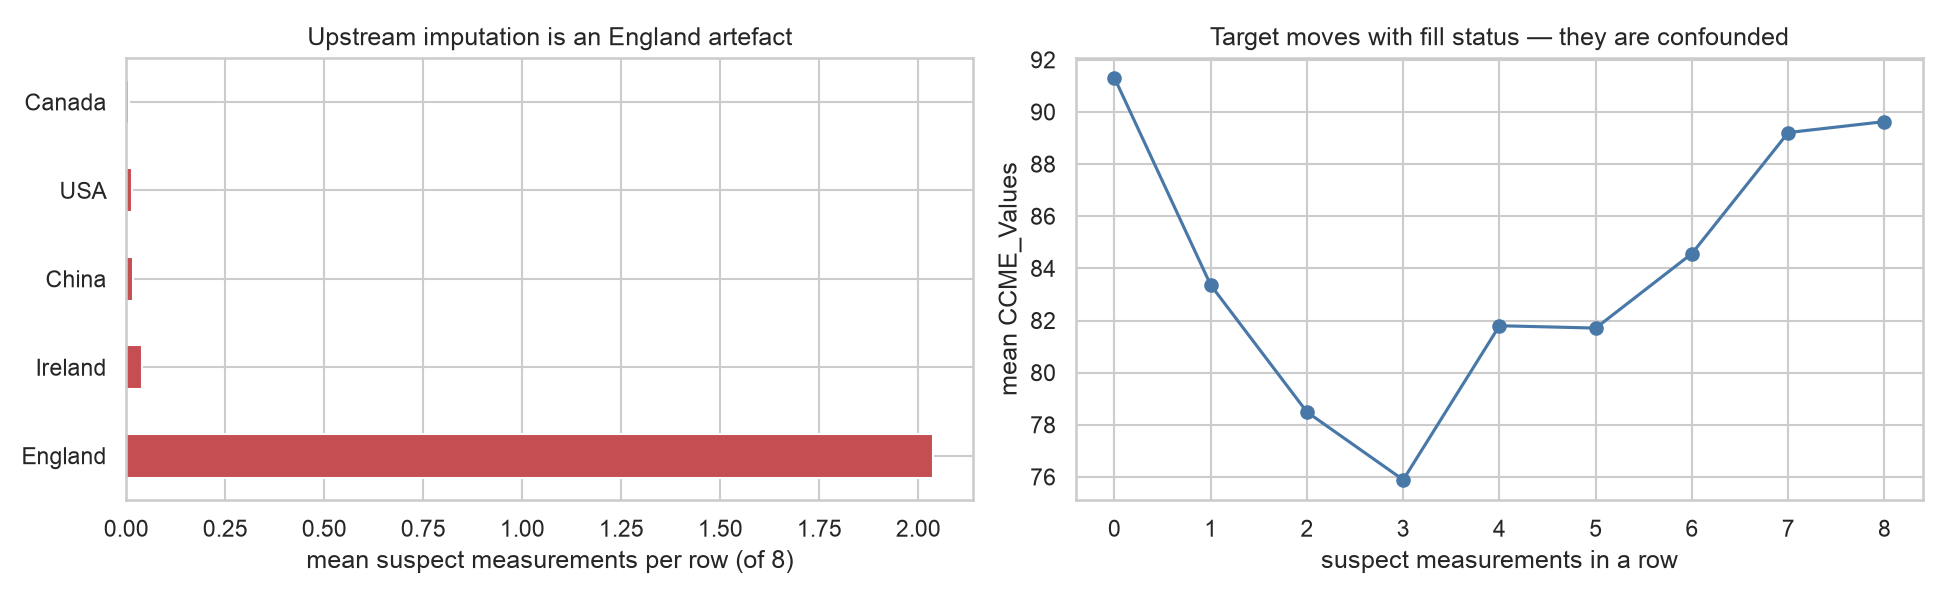
\includegraphics[width=\linewidth]{imputation_confound.png}
    \caption{Upstream median imputation is concentrated in one country (left) and is
    confounded with the target (right). Counts at six or more filled measurements are
    small and the apparent recovery there is noise.}
    \label{fig:imputation}
\end{figure}

\subsection{A Bounded Target with a Mass at the Ceiling}
\label{sec:ceiling}
The index is bounded above at 100 and 35.92\% of records sit exactly at that bound; the
75th, 90th and 99th percentiles are all 100 (Fig.~\ref{fig:target}). The distribution has
no upper tail, only a spike. The share at the ceiling varies from 20.9\% (England) to
84.5\% (USA), so the target's shape differs by country. Residuals above the ceiling are
impossible by construction, making errors asymmetric.

We describe this as a bounded target with a point mass rather than a censored one, and
the distinction matters for how it should be modelled. Censoring implies a latent value
beyond the observation threshold that the recording process conceals. Here there is no
latent value: by Equation~\eqref{eq:ccme}, a record for which every measurement meets its
guideline yields $F_1 = F_2 = F_3 = 0$ and therefore exactly 100. The ceiling is a
property of the index's construction, not of its measurement, so Tobit-style censored
regression is not the appropriate remedy. What the mass does imply is that the task
mixes two questions -- whether a record is fully compliant, and how far from compliance
it falls otherwise -- which a single pooled error statistic reports as one number.

\begin{figure}[!t]
    \centering
    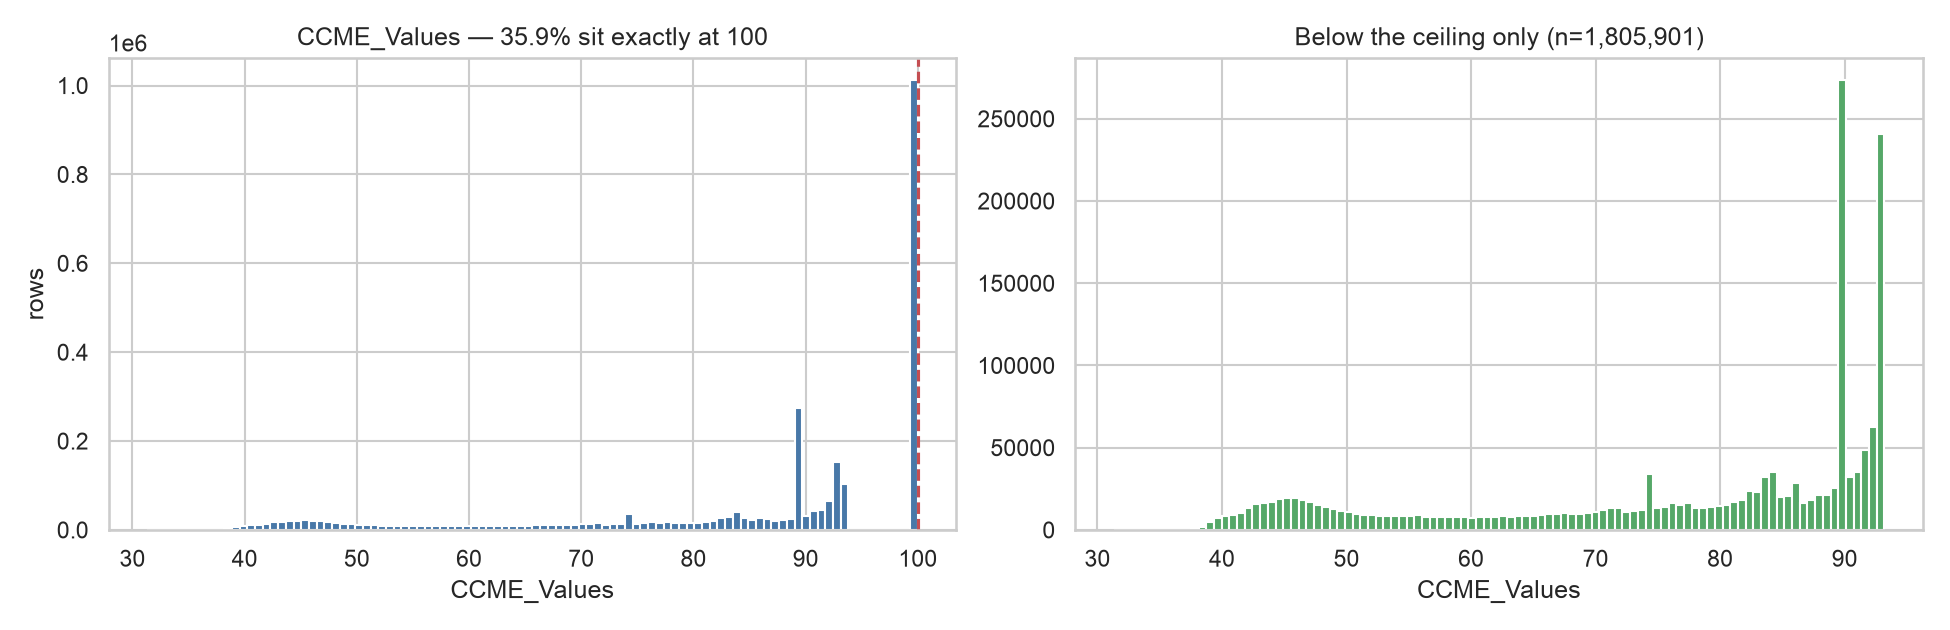
\includegraphics[width=\linewidth]{target_distribution.png}
    \caption{The CCME index is bounded at 100, where 35.92\% of records sit exactly
    (left); the distribution below the ceiling is shown at right.}
    \label{fig:target}
\end{figure}

\subsection{Distributional Properties}
The measurements are strongly right-skewed: ammonia reaches a skewness of 11.98 with
kurtosis 222, BOD 10.21 and orthophosphate 8.94. A $\log(1+x)$ transform reduces ammonia
skewness to 3.35. Tree ensembles are invariant to monotone transforms, so this matters
chiefly for the Phase 2 neural model, but we evaluate the transformed features in
ablation regardless.

Orthophosphate attains a Spearman correlation of $-0.917$ with the target, consistent
with its tight guideline threshold dominating the index excursion term. Dissolved oxygen,
by contrast, correlates almost not at all ($r = -0.031$). As dissolved oxygen is a
``more-is-better'' parameter, this suggests the upstream implementation treats its
guideline as an upper bound; we return to this in Section~\ref{sec:limitations}.

Composition is uneven in two further respects. Effluent and sewage account for 22.1\% of
records -- treatment-works outflow rather than natural surface water -- with a mean index
of 66.6 against 90.0 for rivers. And 82\% of records fall between 2000 and 2019, with
England's series beginning only in 2000.

\section{Methodology}
\label{sec:method}

\subsection{Problem Formulation}
Let $x \in \mathbb{R}^8$ denote the measurement vector -- ammonia, BOD, dissolved oxygen,
orthophosphate, pH, temperature, nitrogen and nitrate -- and $y \in [0,100]$ the CCME
index. The index is defined~\cite{ccme2001wqi} from a scope factor $F_1$, a frequency
factor $F_2$ and an amplitude factor $F_3$ as
\begin{equation}
    y = 100 - \frac{\sqrt{F_1^2 + F_2^2 + F_3^2}}{1.732},
    \label{eq:ccme}
\end{equation}
where $\sqrt{3} \approx 1.732$ normalises the maximum attainable distance to 100. Because
each record in this corpus is an individual measurement rather than an aggregated time
window, the upstream pipeline sets $F_2 \equiv F_1$; we note this adaptation because it
departs from the protocol as published and affects how the index should be read.

Equation~\eqref{eq:ccme} is deterministic in $x$. Learning $f : x \mapsto y$ from the
complete vector is therefore function approximation, and its error is bounded below only
by the capacity of the approximator. We instead study
\begin{equation}
    f_S : x_S \mapsto y, \qquad S \subset \{1,\dots,8\},
    \label{eq:partial}
\end{equation}
where $x_S$ is the measurement vector restricted to an available subset. For
$|S| < 8$ the formula cannot be evaluated, no closed-form solution exists, and the model
must exploit statistical structure among parameters, sites and water body types. We
report $|S| \in \{8,7,6,4\}$ and retain $|S| = 8$ as an emulation benchmark rather than a
prediction result.

The subsets are chosen to be interpretable rather than exhaustive. The 7/8 regime
withholds orthophosphate, which Section~\ref{sec:results} shows to be the dominant driver
of the index; 6/8 additionally withholds BOD, removing the heavy-organics signal; and 4/8
retains only the core physical-chemical suite of pH, dissolved oxygen, temperature and
nitrate, approximating what a continuously deployed in-situ sensor package measures
without laboratory assay.

\subsection{Splitting}
\label{sec:split}
All experiments share one partition, generated once and persisted to disk. Every model at
every availability level is validated and tested on byte-identical records, so reported
differences between models are not attributable to differences in evaluation data. The
training sets differ in size, and we state that explicitly in Section~\ref{sec:models}
rather than claiming a parity we do not have.

Records are grouped by monitoring station (\texttt{Area}, 61{,}689 distinct sites) and
whole groups are allocated to training, validation or test in a $70/15/15$ ratio, with
allocation stratified by country. No site appears in more than one partition. This
follows directly from the concern raised in~\cite{roberts2017cv}: the same station
sampled on consecutive dates yields near-identical chemistry, so a record-level random
split would place near-duplicates on both sides and report a figure that reflects site
memorisation rather than generalisation. Within each country, sites are shuffled under a
fixed seed and assigned by greedy bin-packing in descending size order, each site going
to whichever partition has the largest remaining deficit, which matches the target
proportions as closely as integer site sizes permit.

One country resists this treatment. China contributes a single site (Hou Bay), which
cannot be divided without breaking the zero-leakage guarantee, and is therefore allocated
entirely to training. Chinese records consequently appear in the reported per-country
breakdown as in-sample and are labelled as such; they are not evidence of generalisation.

\subsection{Preprocessing and Features}
The target is isolated before any transformation and never enters the design matrix. All
fitted statistics -- imputer medians, category encodings and scalers -- are learned from
the training partition alone and applied unchanged to validation and test. Masking for a
partial-measurement regime removes the withheld columns and, importantly, any derived
feature computed from them, so that no masked measurement re-enters through a ratio or a
transform.

The raw feature set comprises the available measurements together with country and water
body type. Site identifiers are excluded: with 61{,}689 levels under a site-grouped
split, every test site is unseen by construction, so the variable can only act as noise.
The engineered set adds logarithmic transforms of the skewed measurements -- ammonia,
BOD, nitrate, nitrogen and orthophosphate, whose skewness reaches 11.98 -- and ratios
between chemical parameters. Flags marking upstream-imputed values
(Section~\ref{sec:imputation}) are withheld from the primary feature set and evaluated
separately by ablation, because they are confounded with country.

Programmatic checks assert, for every configuration, that the target does not appear
among the features and that no group spans two partitions.

\subsection{Models and Training Budgets}
\label{sec:models}
Three predictors are compared. A median predictor establishes the floor any model must
clear. Random Forest is tuned over tree count, depth, minimum leaf size and features per
split. XGBoost is tuned over learning rate, depth, subsample, column subsample, minimum
child weight and $L_1$/$L_2$ regularisation, with early stopping on the validation
partition.

The two ensembles are not trained on the same number of records. The partition assigns
1{,}986{,}397 records to training, and XGBoost uses all of them; Random Forest is fitted
on a uniformly drawn subsample of 100{,}000, approximately 5\% of the available training
data. The reason is computational: Random Forest grows unpruned trees whose memory and
fitting cost scale with the number of records retained at every node, and fitting the
full partition was not feasible within our budget, whereas boosting's sequential,
depth-limited trees are far cheaper per record.

This is a genuine asymmetry and we do not want it read as a like-for-like comparison. The
two models see identical validation and test records, identical preprocessing and the
same feature sets, but unequal training data. The reported margin in favour of XGBoost
therefore reflects a combination of algorithmic difference and training budget, and part
of the gap would likely close if Random Forest were given the full partition. We return
to this in Section~\ref{sec:limitations}. Both expose the same training interface so that the Phase 2 neural model can
enter the identical evaluation path. Hyperparameters are selected on validation only; the
test partition is evaluated once, at the end.

\subsection{Metrics}
We report mean absolute error, root mean squared error and the coefficient of
determination, computed through a single shared implementation so that every model is
scored identically. MAE is reported alongside RMSE because the two respond differently to
the heavy tails documented in Section~\ref{sec:data}: RMSE is dominated by the small
number of large excursions, while MAE describes the typical record. $R^2$ is reported for
comparability with the water quality literature, with the caveat that its baseline is the
target variance, which differs across availability regimes.

Confidence intervals are obtained by bootstrap resampling of the test partition, which
makes the comparison between models a statement about sampling variability rather than a
single point estimate. As noted in Section~\ref{sec:ceiling}, the target is bounded above
and carries a large point mass at that bound; the metrics reported here are pooled across
it, and Section~\ref{sec:limitations} states what that conflates.

\section{Experiments and Results}
\label{sec:results}

\subsection{Baseline and Full-Measurement Benchmark}
Table~\ref{tab:main} reports the three models under full measurement availability. The
median baseline attains $R^2 = -0.092$, confirming that a constant predictor is worse
than useless on this target. Both ensembles exceed it by a wide margin, with XGBoost
reaching $R^2 = 0.9997$ and a mean absolute error of 0.100 index points. Throughout, the
two ensembles are trained on unequal budgets -- Random Forest on a 100{,}000-record
subsample, XGBoost on the full 1{,}986{,}397-record partition
(Section~\ref{sec:models}) -- so the margin between them is not a clean algorithmic
comparison and should be read with that in mind.

This near-perfect score should be read as what it is. By Equation~\eqref{eq:ccme} the
target is determined by the inputs, so the result measures how well a tree ensemble
approximates a known piecewise function. We report it as a benchmark and as a check on
the pipeline: a materially lower score here would indicate a defect upstream.

\begin{table}[!t]
    \centering
    \caption{Phase 1 model comparison on the held-out test set, all-measurements regime; all figures are test-set. The baseline predicts the training median; Random Forest is fitted on a 100k subsample and XGBoost on the full training partition, both with engineered features.}
    \label{tab:main}
    \small
    \setlength{\tabcolsep}{4pt}
    \begin{tabular}{lrrrr}
        \toprule
        Model & MAE & RMSE & $R^2$ & Train (s) \\
        \midrule
        Naive baseline & 13.605 & 19.492 & -0.0923 & 0.0 \\
        Random Forest & 0.408 & 0.920 & 0.9976 & 1.7 \\
        XGBoost & 0.100 & 0.328 & 0.9997 & 49.3 \\
        \bottomrule
    \end{tabular}
\end{table}


\subsection{Partial Measurement Availability}
Table~\ref{tab:partial} and Fig.~\ref{fig:degradation} give the central result.
Withholding a single measurement moves XGBoost from $R^2 = 0.9997$ to $0.834$, and mean
absolute error from 0.100 to 4.776 -- a factor of 48. Withholding four leaves
$R^2 = 0.573$ and an error of 8.596 index points, which spans roughly one CCME quality
class. XGBoost leads Random Forest at every level, and the margin is stable at
2--4\% of $R^2$ despite the twentyfold difference in training-set size, which suggests
the ordering is not purely a budget effect even though its magnitude is not separable
from one.

The gap between the 8/8 and 7/8 rows is the quantitative statement of the leakage
problem. Almost all of the apparent accuracy in the full-measurement setting comes from
the formula being reconstructible, not from any learned relationship that survives when
an input is withdrawn.

\begin{table*}[!t]
    \centering
    \caption{Degradation under partial measurement availability. The 8/8 row is a formula-emulation benchmark, not independent prediction; genuine estimation begins at 7/8. $p$ is the feature count after masking; all figures are test-set.}
    \label{tab:partial}
    \small
    \setlength{\tabcolsep}{4pt}
    \begin{tabular}{llrrrr}
        \toprule
        Avail. & Model & $p$ & MAE & RMSE & $R^2$ \\
        \midrule
        8/8 & Random Forest & 38 & 0.408 & 0.920 & 0.9976 \\
        8/8 & XGBoost & 23 & 0.100 & 0.328 & 0.9997 \\
        7/8 & Random Forest & 35 & 5.328 & 8.145 & 0.8093 \\
        7/8 & XGBoost & 20 & 4.776 & 7.597 & 0.8341 \\
        6/8 & Random Forest & 32 & 5.675 & 8.544 & 0.7901 \\
        6/8 & XGBoost & 17 & 5.209 & 8.045 & 0.8139 \\
        4/8 & Random Forest & 25 & 9.305 & 12.781 & 0.5304 \\
        4/8 & XGBoost & 10 & 8.596 & 12.190 & 0.5728 \\
        \bottomrule
    \end{tabular}
\end{table*}


\begin{figure}[!t]
    \centering
    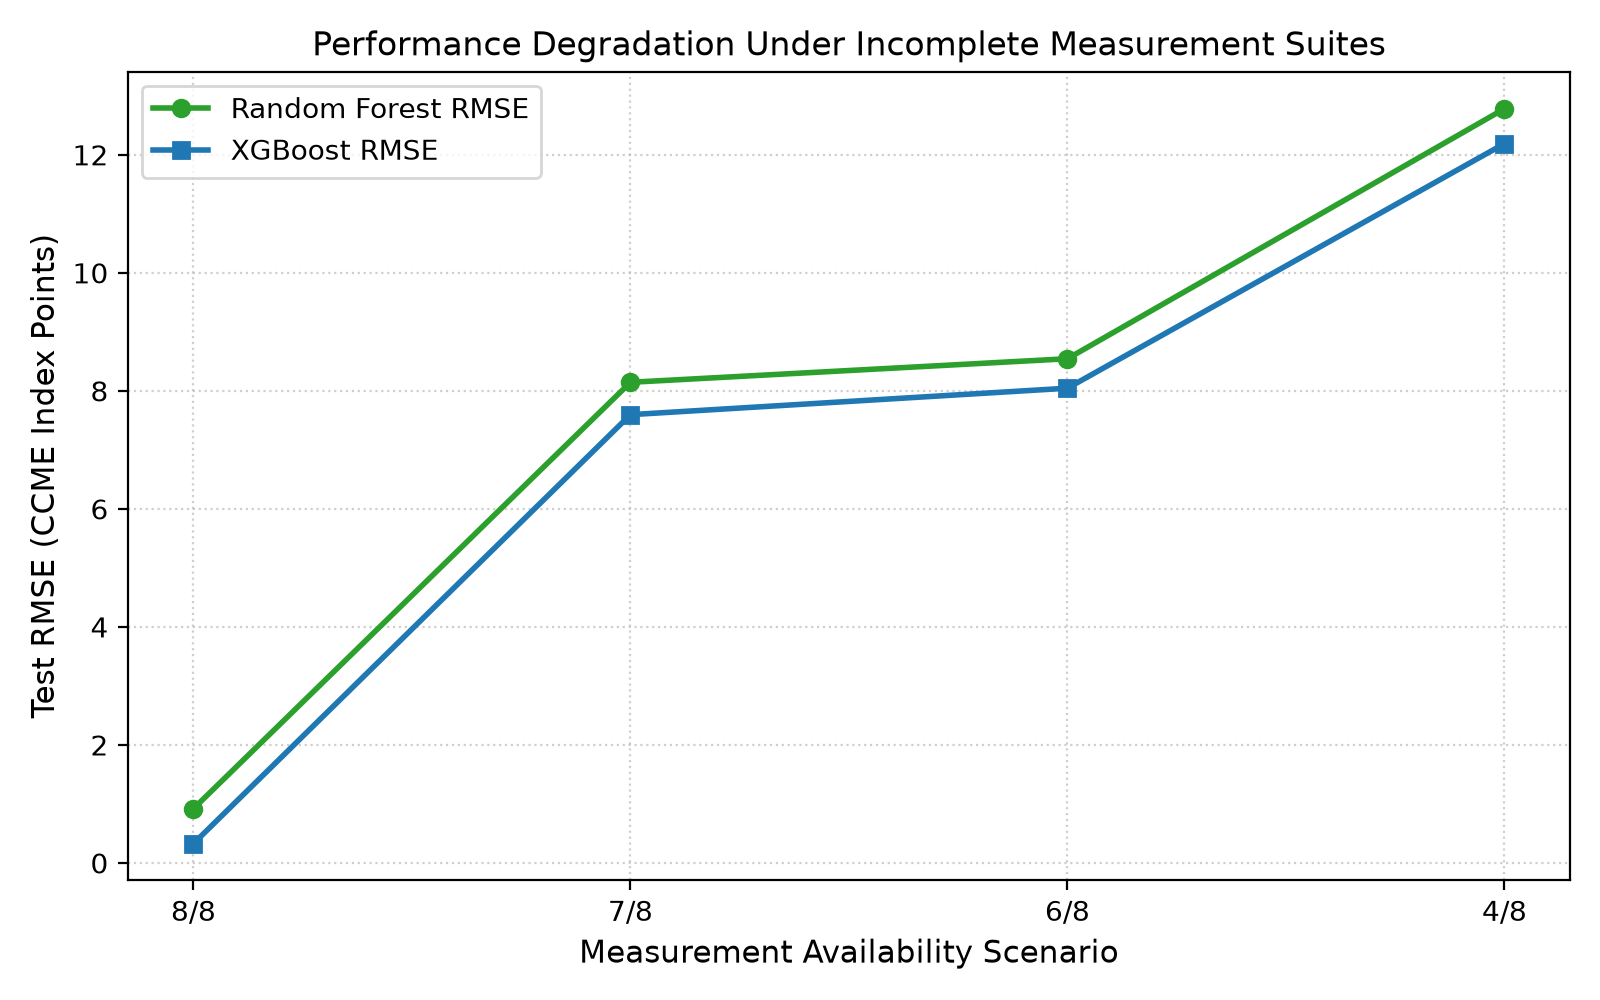
\includegraphics[width=\linewidth]{06_partial_measurement_degradation.png}
    \caption{Test performance against measurement availability. The step between 8/8 and
    7/8 isolates the contribution of formula reconstruction.}
    \label{fig:degradation}
\end{figure}

\subsection{Ablations}
Table~\ref{tab:ablation} isolates two design choices. Engineered features reduce XGBoost
test MAE from 0.1517 to 0.1000, a 34\% relative improvement, confirming that the
logarithmic transforms and chemical ratios carry information beyond the raw columns.
Adding the upstream-imputation flags changes test MAE only from 0.1517 to 0.1474. Given
their confounding with country (Section~\ref{sec:imputation}), this small gain does not
justify their inclusion, and we exclude them from the primary configuration.

\begin{table*}[!t]
    \centering
    \caption{Ablation studies on XGBoost, all-measurements regime. $p$ is the feature count; all figures are test-set.}
    \label{tab:ablation}
    \small
    \setlength{\tabcolsep}{4pt}
    \begin{tabular}{lllrrr}
        \toprule
        Ablation & Config. & $p$ & MAE & RMSE & $R^2$ \\
        \midrule
        Imputation flags & Excluded (primary) & 10 & 0.1517 & 0.4005 & 0.99954 \\
        Imputation flags & Included & 20 & 0.1474 & 0.3979 & 0.99954 \\
        Features & Raw & 10 & 0.1517 & 0.4005 & 0.99954 \\
        Features & Raw + engineered & 23 & 0.1000 & 0.3282 & 0.99969 \\
        \bottomrule
    \end{tabular}
\end{table*}


\subsection{Uncertainty and Error Decomposition}
Table~\ref{tab:bootstrap} gives bootstrap confidence intervals. The intervals for Random
Forest and XGBoost do not overlap on any metric, so the ordering between them is not an
artefact of sampling.

Table~\ref{tab:country} decomposes test error by country over all 415{,}804 test
records. Performance is uniformly high in the full-measurement regime, but the sample
sizes are extremely unequal: England supplies 76.8\% of test records and Canada 0.14\%,
so the Canadian figures rest on 584 records and should not be read as a country-level
comparison. England's share of the test set (76.8\%) differs slightly from its share of
the corpus (75.3\%) because whole sites are allocated to partitions, so the split
matches the target proportions only as closely as integer site sizes permit. China is
absent: its single site is allocated wholly to training (Section~\ref{sec:split}), so it
contributes no test records and cannot be evaluated out-of-sample.

\begin{table*}[!t]
    \centering
    \caption{Bootstrap point estimates with 95\% confidence intervals on the test set.}
    \label{tab:bootstrap}
    \small
    \setlength{\tabcolsep}{4pt}
    \begin{tabular}{lllp{0.28\linewidth}}
        \toprule
        Model & MAE (Point [95\% CI]) & RMSE (Point [95\% CI]) & R2 (Point [95\% CI]) \\
        \midrule
        Naive Baseline & 13.6047 [13.5631, 13.6457] & 19.4916 [19.4378, 19.5410] & -0.0923 [-0.0936, -0.0907] \\
        Random Forest & 0.4078 [0.4053, 0.4103] & 0.9197 [0.9102, 0.9297] & 0.9976 [0.9975, 0.9976] \\
        XGBoost & 0.1000 [0.0991, 0.1009] & 0.3282 [0.3228, 0.3337] & 0.9997 [0.9997, 0.9997] \\
        \bottomrule
    \end{tabular}
\end{table*}

\begin{table}[!t]
    \centering
    \caption{Test error decomposed by country, over all 415{,}804 test records. China is absent by construction: its single site (Hou Bay) is allocated wholly to training, so it contributes no test records and cannot be evaluated out-of-sample.}
    \label{tab:country}
    \small
    \setlength{\tabcolsep}{4pt}
    \begin{tabular}{lrrrrr}
        \toprule
        Country & $n$ & \% of test & MAE & RMSE & $R^2$ \\
        \midrule
        England & 319184 & 76.76 & 0.116 & 0.329 & 0.9997 \\
        USA & 60787 & 14.62 & 0.062 & 0.394 & 0.9937 \\
        Ireland & 35249 & 8.48 & 0.019 & 0.123 & 0.9996 \\
        Canada & 584 & 0.14 & 0.176 & 0.561 & 0.9982 \\
        \bottomrule
    \end{tabular}
\end{table}


\subsection{Feature Attribution}
Table~\ref{tab:shap} ranks features by mean absolute SHAP value. Orthophosphate dominates
at 8.813, nearly three times the next contributor, which matches both its Spearman
correlation of $-0.917$ and its position in Equation~\eqref{eq:ccme}: it carries the
tightest guideline threshold and therefore the largest excursion term. The appearance of
the engineered logarithmic transforms in the top five corroborates the ablation.

\begin{table}[!t]
    \centering
    \caption{Ten most influential features by mean absolute SHAP value (XGBoost, 8/8 regime).}
    \label{tab:shap}
    \small
    \setlength{\tabcolsep}{4pt}
    \begin{tabular}{lr}
        \toprule
        Feature & Mean $|$SHAP$|$ \\
        \midrule
        Orthophosphate (mg/l) & 8.813 \\
        log\_Orthophosphate & 3.062 \\
        Ammonia (mg/l) & 2.455 \\
        Biochemical Oxygen Demand (mg/l) & 1.061 \\
        log\_Ammonia & 0.691 \\
        Nitrogen (mg/l) & 0.267 \\
        pH (ph units) & 0.229 \\
        log\_BOD & 0.178 \\
        Temperature (cel) & 0.160 \\
        N\_P\_ratio & 0.110 \\
        \bottomrule
    \end{tabular}
\end{table}


\begin{figure}[!t]
    \centering
    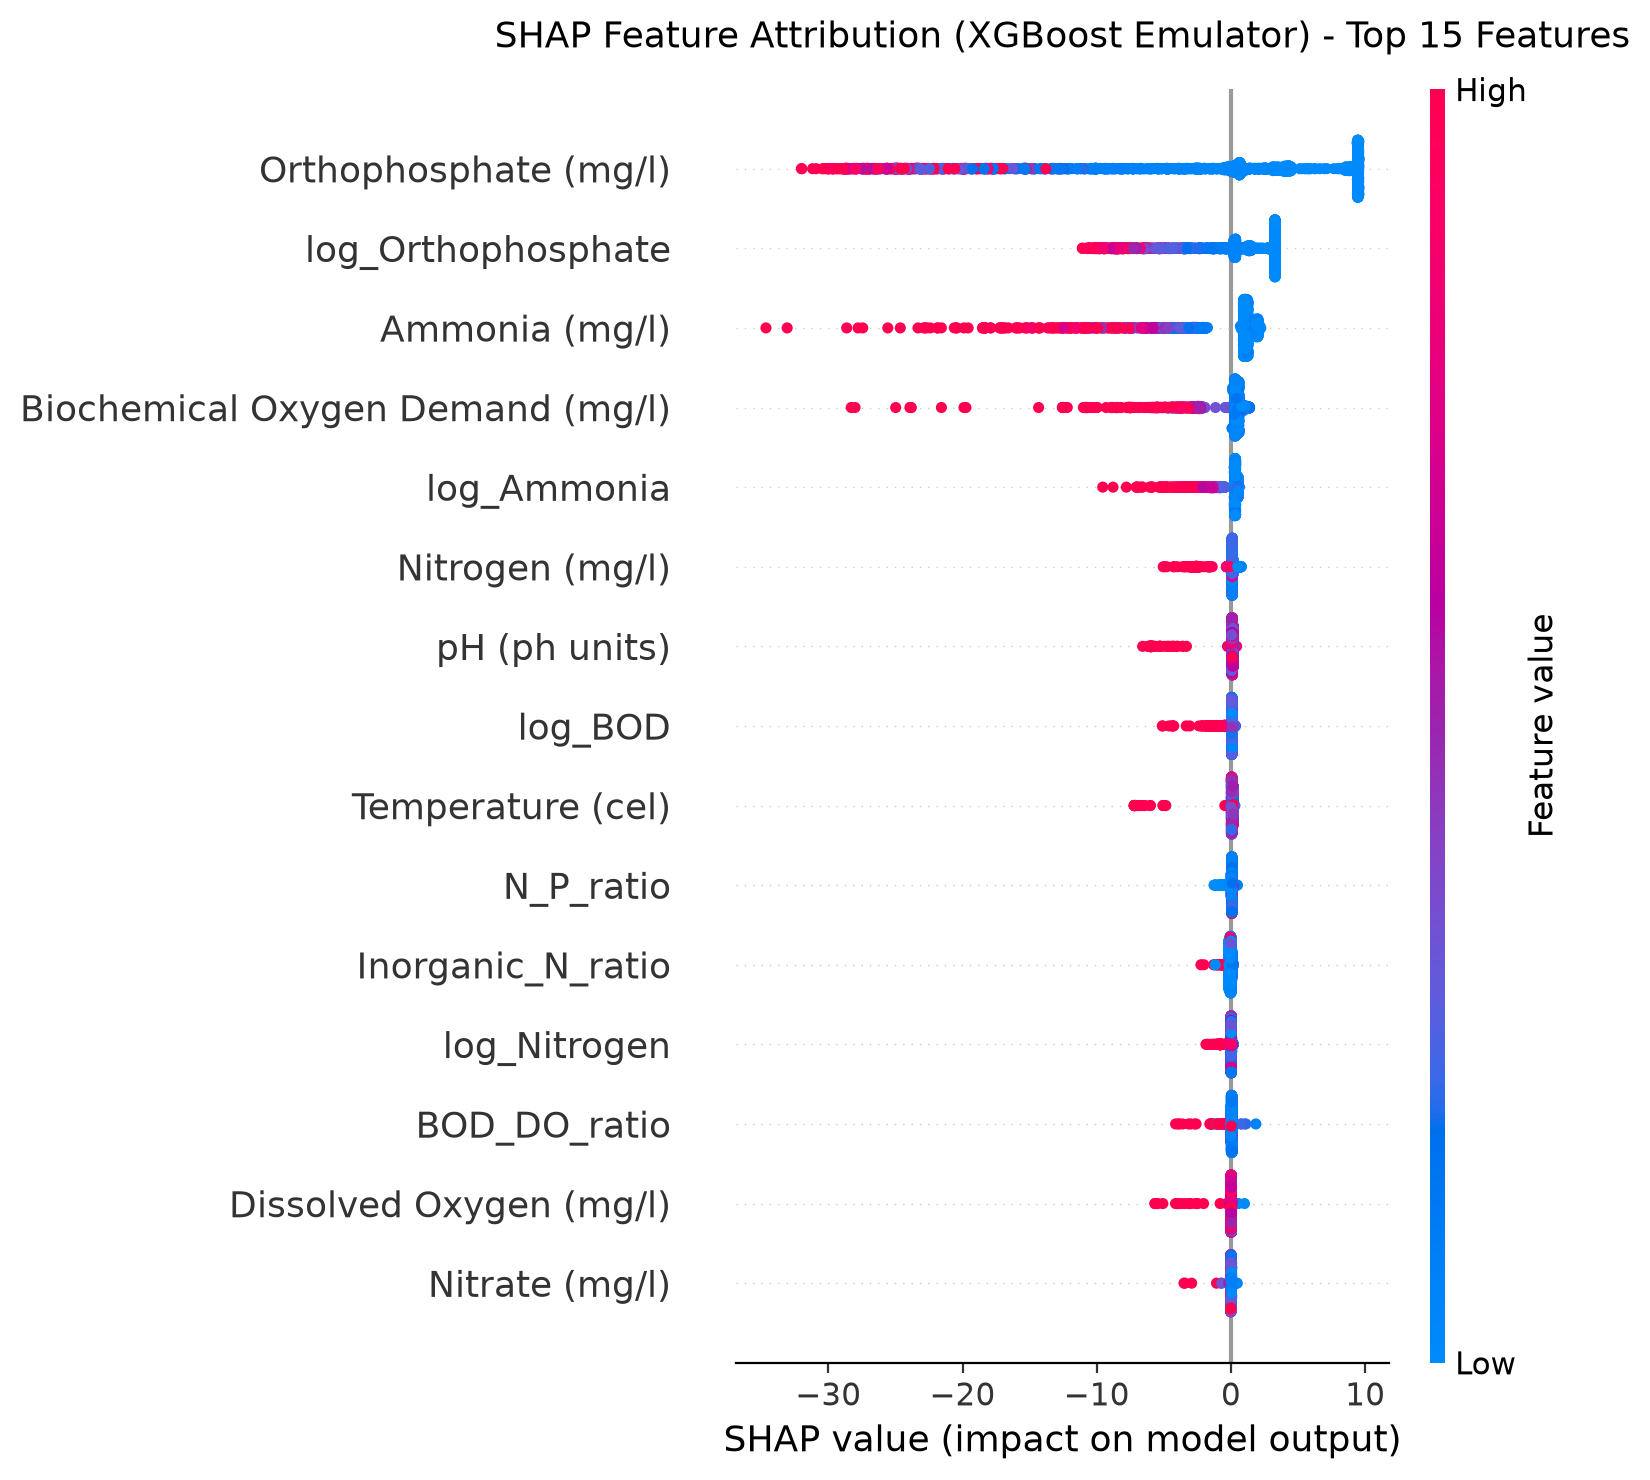
\includegraphics[width=\linewidth]{06_shap_summary.png}
    \caption{SHAP summary for the full-measurement XGBoost model.}
    \label{fig:shap}
\end{figure}

\section{Limitations}
\label{sec:limitations}

\paragraph{Target leakage is mitigated, not eliminated}
The 8/8 regime reconstructs the index formula and we report it as a benchmark rather
than a prediction result. Even at 7/8 and 6/8, the retained measurements are formula
contributors, so part of the remaining performance is partial formula reconstruction
rather than environmental inference. A fully independent regime -- predicting the index
from metadata and spatiotemporal context alone, with no formula contributors -- would
bound this, and we did not run it.

\paragraph{A point mass at the ceiling is reported as one number}
With 35.92\% of records at the upper bound, pooled $R^2$ and RMSE conflate two tasks:
identifying records that are fully guideline-compliant, and estimating how far the
remainder fall short. The figures reported here are pooled. Metrics separated by ceiling
status would characterise the models more honestly, particularly in the low-availability
regimes where identifying compliance is likely the easier half of the problem. We note
that this is a bounded target rather than a censored one
(Section~\ref{sec:ceiling}): no latent value exists above 100, so the remedy is
stratified reporting, not a censored-regression estimator.

\paragraph{Imputation cannot be undone}
Up to 31.6\% of individual measurement columns were median-filled before publication
(Section~\ref{sec:imputation}). The original missingness pattern is unrecoverable, so the
mechanism cannot be classified as MCAR, MAR or MNAR. Because the fill is concentrated in
England, fill status, country and target are mutually confounded, and no split design
removes this.

\paragraph{A probable defect in the upstream index}
Dissolved oxygen correlates with the target at $r = -0.031$. Dissolved oxygen is a
``more-is-better'' parameter and would normally be among the most informative inputs. The
upstream implementation appears to treat its guideline as an upper bound to remain below,
inverting its contribution. We report the index as published and flag this rather than
silently correcting it.

\paragraph{Composition and coverage}
Effluent and sewage comprise 22.1\% of records, so the dataset is not purely natural
surface water. England supplies 75.3\% of records and its series begins in 2000, so the
corpus is not geographically or temporally balanced, and aggregate metrics are dominated
by one country.

\paragraph{What the split does and does not establish}
Because whole monitoring stations are allocated to a single partition, every test record
comes from a site the model has never seen, and the reported figures are therefore
estimates of generalisation to new stations. They are not estimates of generalisation
across time: the split is not chronological, so a test site's records may fall in the
same period as the training data, and nothing here speaks to extrapolation into future
years or to conditions outside the observed range. The Chinese subset is a further
exception, being single-site and allocated entirely to training
(Section~\ref{sec:split}); its per-country figures are in-sample.

\paragraph{Unequal training budgets}
Random Forest is fitted on a 100{,}000-record subsample while XGBoost uses the full
1{,}986{,}397-record training partition (Section~\ref{sec:models}). Validation and test
records, preprocessing and feature sets are identical, but the training data is not. The
margin reported in favour of XGBoost therefore confounds algorithmic capability with
training-set size, and should be read as an upper bound on the true algorithmic gap.
Equalising the budgets is the first experiment we would add.

\paragraph{China cannot be evaluated out-of-sample}
China contributes a single monitoring site, which cannot be divided across partitions
without breaking the grouping guarantee and is therefore allocated wholly to training. It
contributes no test records and is absent from Table~\ref{tab:country}. Nothing in this
paper evidences performance on Chinese waters.

\paragraph{Subset selection}
The four availability regimes are interpretable rather than exhaustive. There are eight
ways to withhold one measurement and seventy ways to withhold four; we report one
informative choice at each level rather than averaging over all of them. The degradation
curve should therefore be read as evidence that performance collapses once formula
reconstruction is impossible, not as a precise estimate of expected loss under arbitrary
missingness.

\section{Conclusion}
\label{sec:conclusion}

We set out to predict the CCME Water Quality Index from physical and chemical
measurements and found that the conventional framing of that task does not survive
examination. The index is a deterministic function of the measurements that define it, so
a model given all eight recovers a formula rather than learning anything about water
quality. Measured directly, this framing yields $R^2 = 0.9997$ and a mean absolute error
of 0.100 index points -- figures that look like a result and are not one. We report them
only as an emulation benchmark and as a check that the pipeline is sound.

Reframing the problem as estimation under partial measurement availability restores its
content. Withholding orthophosphate alone moves XGBoost to $R^2 = 0.834$ and multiplies
error by a factor of 48; withholding half the measurements leaves $R^2 = 0.573$ and an
error of 8.596 index points, roughly the width of one CCME quality class. The step
between the full and partial regimes is the quantitative statement of how much apparent
accuracy was reconstruction rather than inference. Within this formulation XGBoost leads Random
Forest at every availability level, on identical test records and preprocessing, by a
margin that bootstrap intervals confirm is not a sampling artefact -- though the two were
trained on unequal budgets, so that margin bounds rather than measures the algorithmic
difference. Engineered
logarithmic and ratio features reduce error by 34\%, while flags marking upstream
imputation, being confounded with country, do not earn inclusion.

Two findings extend beyond this dataset. The first is that a published, reusable corpus
reporting no missing values had in fact been median-imputed before release, in a pattern
detectable only from the modal structure of its columns and concentrated almost entirely
in one contributing country. The second is that dissolved oxygen, which should be among
the most informative parameters in any water quality assessment, carries almost no
relationship to the index as distributed -- consistent with its guideline being applied in
the wrong direction upstream. Both were found by examining the data rather than the
documentation, and both would have been invisible to a study that reported only
predictive accuracy.

Phase 2 extends this work to a regularised multilayer perceptron trained on the same
partitions and preprocessing, which allows the tree ensembles and the neural model to be
compared without the confounds that make such comparisons unreliable in the literature.
The skewness documented in Section~\ref{sec:data} is expected to matter there in a way it
does not for trees, since neural models are not invariant to monotone transforms, and the
engineered features will be ablated accordingly. The point mass at the target's ceiling also
deserves direct treatment, through metrics separated by compliance status and potentially
through a model that represents the boundary explicitly rather than regressing through
it.


\bibliographystyle{IEEEtran}
\bibliography{../docs/refs}

\end{document}
